\section{Dátový model}
Z dôvodu rozšíriteľnosti aplikácie zavádzame \textbf{používateľské role} ako \textit{abstraktné entity}, ktoré môžu byť definované pomocou systému oprávnení. 
Každá rola bude mať priradené určité oprávnenia, ktoré určujú, aké akcie môže používateľ s danou rolou vykonávať v aplikácii. 
Tento prístup nám umožní flexibilne pridávať nové role a oprávnenia bez nutnosti zásahu do základnej štruktúry systému.

\vspace{1em}\hspace{-2em}
Všeobecne bude \textit{Nájomca}, \textit{Majiteľ nehnuteľnosti} a \textit{Administrátor} definovaný ako \textbf{User} s príslušnými oprávneniami.

\vspace{1em}\hspace{-2em}
Dátový model taktiež definuje prácu so súbormi, ktoré môžu byť pripojené k rezerváciám alebo nehnuteľnostiam (zatiaľ iba ako obrázky).

\vspace{1em}\hspace{-2em}
Entitno-relačný diagram (ERD) znázorňujúci vzťahy medzi entitami v našom systéme je uvedený nižšie.

\vspace{1em}\hspace{-2em}
\textit{Poznámka: Anotácia typu napr. PK+FK znamená, že dané atributy sú PK aj FK.}

\vspace{0.5em}\hspace{-2em}
\textit{Podobne, UNI+FK znamená, že dané atributy sú v kombinácii UNIQUE a každý z nich je FK, ale UNI (+FK) znamená, že dané atribúty sú v kombinácii UNIQUE, ale FK je iba atribút na úrovni 'newline' (+FK).}

\vspace{0.5em}\hspace{-2em}
\textit{Teda riadok anotovaný UNI sa viaže na kombináciu atribútov, (.*) na úroveň 'newline' a iné nevytvárajú kombinácie, ale hovoria o vlastnosti pre každý atribút zvlášť.}

\begin{figure}[ht!]\centering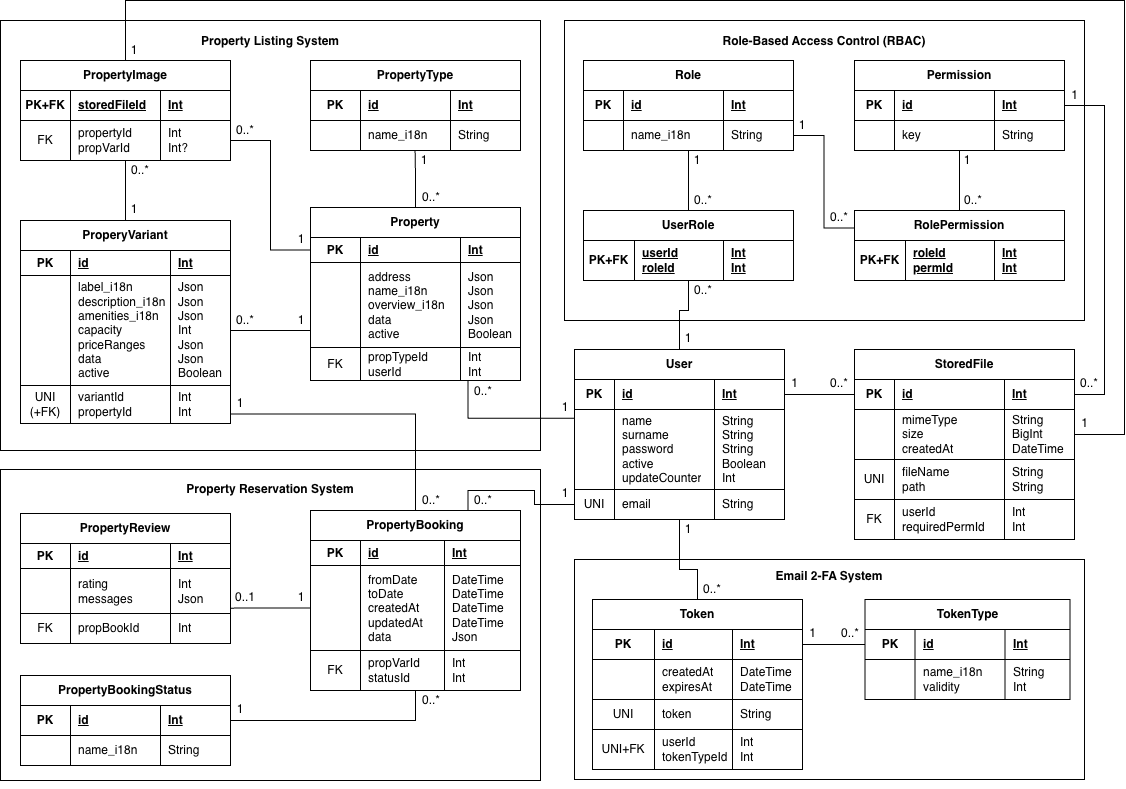
\includegraphics[width=\textwidth]{images/dm-er.png}\end{figure}


\subsection{Popis entít}

\paragraph{User} \text{ } \newline
Vyjadruje používateľa systému, ktorý môže byť \textit{Nájomca}, \textit{Majiteľ nehnuteľnosti} alebo \textit{Administrátor}. 
Obsahuje štandardné atribúty ako \textit{name, surname, password} a navyše:
\begin{itemize}[itemsep=2pt]
    \item \textit{email} - jednoznačný identifikátor používateľa (používaný pre prihlásenie),
    \item \textit{active} - identifikuje, či je daný účet aktivný,
    \item \textit{updateCounter} - identifikuje počet aktualizácii profilu, ktoré vynútia odhlásenie používateľa a opätovné prihlásenie (napr. zmena hesla) na ostatých zariadeniach.
\end{itemize}

\paragraph{StoredFile} \text{ } \newline
Reprezentuje súbor uložený v systéme, ktorý môže byť pripojený k nehnuteľnostiam ako obrázok.
Obsahuje nasledujúce atribúty:
\begin{itemize}[itemsep=2pt]
    \item \textit{mimeType, size, createdAt} - udržiavanie typu, veľkosti súbora a času vytvorenia,
    \item \textit{filename, path} - jednoznačné identifikátory súbora (v kombinácii UNIQUE),
    \item \textit{userId, requiredPermId} - foreign kľúče pre identifikáciu vlastníka súboru a potrebného oprávnenia pre prístup k súboru.
\end{itemize}

\paragraph{Token} \text{ } \newline
Reprezentuje autentifikačný token, ktorý je používaný pre autentifikáciu a autorizáciu používateľov v systéme. 
Používa sa napríklad pri zmene hesla alebo aktivácii účtu, ktorý uživateľ dostane na svoju emailovú adresu s obmedzenou platnosťou.
Obsahuje nasledujúce atribúty:
\begin{itemize}[itemsep=2pt]
    \item \textit{createdAt, expiresAt} - čas vytvorenia a expirácie tokenu,
    \item \textit{token, tokenTypeId, userId} - konkrétna textová reprezentácia tokenu, typ tokenu a foreign kľúč pre identifikáciu vlastníka tokenu.
\end{itemize}
Navyše \textit{token}, ale aj kombinácia \textit{(tokenTypeId, userId)} musia byť UNIQUE, pretože každý používateľ môže mať len jeden aktívny token daného typu a zároveň by nemal existovať reťazec tokenu, ktorý je spoločný pre viacerých userov.

\paragraph{TokenType} \text{ } \newline
Reprezentuje konkrétny typ tokenu, ktorý môže byť použitý, obsahuje atribúty ako:
\begin{itemize}[itemsep=2pt]
    \item \textit{name\_i18n} - lokalizovaný názov typu tokenu,
    \item \textit{validity} - doba platnosti tokenu v sekundách.
\end{itemize}

\paragraph{Role} \text{ } \newline
Reprezentuje rolu, ktorá môže mať priradené určité oprávnenia s atribútom \textit{name\_i18n}, ktorý obsahuje lokalizovaný názov role.

\paragraph{UserRole} \text{ } \newline
Definuje vzťah medzi používateľom a rolou, ktorá určuje, aké oprávnenia má použivateľ v rámci danej role.
Atribútami sú \textit{userId, roleId}, ktoré sú primary kľúče a zároveň aj foreign kľúčami.

\paragraph{Permission} \text{ } \newline
Definuje oprávnenie s atribútom \textit{key}, ktorý identifikuje dané oprávnenie.

\paragraph{RolePermission} \text{ } \newline
Definuje vzťah medzi rolou a oprávnením, ktorý určuje, aké oprávnenia má daná rola.
Atribútami sú \textit{roleId, permId}, ktoré sú primary kľúče a zároveň aj foreign kľúčami.

\paragraph{Property} \text{ } \newline
Reprezentuje konkrétnu nehnuteľnosť, ktorá môže mať viac variant (ak nemá žiadnu, nie je možné ju zviditeľniť - active == false).
Obsahuje nasledujúce atribúty:
\begin{itemize}[itemsep=2pt]
    \item \textit{address, name\_i18n, overview\_i18n} - adresa, lokalizovaný názov a popis nehnuteľnosti,
    \item \textit{data} - voliteľné pole pre uloženie ďalších informácií o nehnuteľnosti,
    \item \textit{active} - identifikuje, či je nehnuteľnosť aktívna (zobrazuje sa),
    \item \textit{propTypeId, userId} - foreign kľúče pre identifikáciu typu nehnuteľnosti (byt, hotel, atd.) a vlastníka nehnuteľnosti.
\end{itemize}

\paragraph{PropertyType} \text{ } \newline
Reprezentuje typ nehnuteľnosti, ktorý môže byť použitý pre kategorizáciu nehnuteľností a obsahuje atribút \textit{name\_i18n}, ktorý obsahuje lokalizovaný názov typu nehnuteľnosti.

\paragraph{PropertyVariant} \text{ } \newline
Reprezentuje variant nehnuteľnosti (izba v hoteli, konkrétny apartmán alebo konkrétny priestor v rámci nehnuteľnosti).
Obsahuje nasledujúce atribúty:
\begin{itemize}[itemsep=2pt]
    \item \textit{label\_18n, description\_18n, amenities\_i18n} - lokalizovaný názov, popis variantu a vybavenia variantu,
    \item \textit{capacity} - maximálny počet osôb, ktorý môže byť v tomto variante ubytovaných (iba pre "bytové jednotky"),
    \item \textit{priceRanges} - pole pre uloženie ceny prenájmu vo formáte (od, do, cena/noc, [príplatky]),
    \item \textit{data} - voliteľné pole pre uloženie ďalších informácií o variante,
    \item \textit{active} - identifikuje, či je tento variant aktivný (zobrazuje sa),
    \item \textit{variantId, propertyId} - jednoznačná kombinácia čísla variantu (1..*) a foreign kľúca pre identifikáciu nehnuteľnosti, ktorej tento variant patrí.
\end{itemize}

Cena rezervácie sa vypočíta na \textit{priceRanges} súčtom cien za noc pre dané dátumové rozmedzie a (voliteľné) príplatkov.
(Voliteľné) Príplatky môžu byť definované administrátorom: napr. cena na osobu / dieta, cena za upratovanie, parkovanie a podobne (budú vyžadovať rozšírenie dátového modelu).

\paragraph{PropertyImage} \text{ } \newline
Reprezentuje obrázok pripojený ku konkrétnemu alebo všetkým variantom nehnuteľnosti.
Obsahuje nasledujúce atribúty:
\begin{itemize}
    \item \textit{storedFileId} - primary a zároveň aj foreign kľúč pre identifiaciu súboru,
    \item \textit{propertyId} - foreign kľúč pre identifikáciu nehnuteľnosti, ktorej tento obrázok patrí,
    \item \textit{propVarId} - nullable foreign kľúč pre identifikáciu konkrétneho variantu, ktorému tento obrázok patrí (ak je null, patrí každému variantu nehnuteľnosti).
\end{itemize}



\paragraph{PropertyBooking} \text{ } \newline
Reprezentuje konkrétnu rezerváciu variantu nehnuteľnosti konkrétnym používateľom. Po jej absoľvovaní umožní pridať k nehnuteľnosti recenziu.
Obsahuje nasledujúce atribúty:
\begin{itemize}[itemsep=2pt]
    \item \textit{fromDate, toDate, createdAt, updatedAt} - dátum začiatku a konca rezervácie, dátum vytvorenia rezervácie a dátum aktualizácie rezervácie,
    \item \textit{data} - voliteľné pole pre uloženie ďalších informácií o rezervacií,
    \item \textit{propVarId, statusId} - foreign kľúče identifikujúce variant nehnuteľnosti a stav rezervácie.
\end{itemize}

\paragraph{PropertyBookingStatus} \text{ } \newline
Reprezentuje stav rezervácie, ktorý môže byť použitý pre identifikáciu aktuálneho stavu (napr. "potvrdená", "zrušená", ...).
Obsahuje atribút \textit{name\_i18n}, ktorý obsahuje lokalizovaný názov stavu rezervácie.

\paragraph{PropertyReview} \text{ } \newline
Reprezentuje recenziu, ktorá môže byť priradená ku už absolvovanej rezervacií variantu nehnuteľnosti.
Obsahuje následujúce atribúty:
\begin{itemize}[itemsep=2pt]
    \item \textit{rating} - hodnotenie variantu nehnuteľnosti v rozsahu 1..5,
    \item \textit{messages} - json pole pre uloženie správ recenzie medzi nájomcom a majitelom nehnuteľnosti; formát \textit{(userId: Integer, createdAt: DateTime, updatedAt: DateTime, message: String)}, pričom musí existovať a zároveň byť prvá správa od nájomcu.
    \item \textit{propBookId} - foreign kľúč pre identifikáciu rezervácie, ku ktorej je recenzie priradená.
\end{itemize}